%% présentation générale
%% architecture





\begin{frame}{Introduction}

  \begin{block}{Système de Réécriture}

    Une méthode pour modéliser de façon générale les opérations de
    remplacement de sous-termes par d'autres.
    ~\\

    \emph{ie. etape de réduction pour la semantique d'un language,
      Lois de De Morgan en logique propositionnelle, arithmétique de Peano}
    
  \end{block}

  
\end{frame}

\begin{frame}{Système de Réécriture}

  \begin{block}{Definition}
    
    \begin{itemize}
      \item un ensemble de termes 
      \item un ensemble de règles (terme * terme)
    \end{itemize}

  \end{block}

  réécrire un terme : appliquer les règles conformément à une
  \textcolor{red}{stratégie} prédéfinie sur un term donné en
  \emph{matchant} et en replaçant ses sous-termes.

  ~\\
  Par exemple : \\
  Rule : \texttt{Sub(Add(X))} $\rightarrow$ \texttt{X}\\
  ~\\
  \textcolor{blue}{\texttt{Sub(Add(0))}} $ \rightarrow $ \textcolor{blue}{\texttt{0}}

\end{frame}


\begin{frame}{Réécriture Nominale Non Linéaire}
  
  \begin{block}{Nominale}
    Il existe une distinction entre atomes (variables du langage) et
    méta-variables/placeholders (sous-termes à remplacer).
  \end{block}

  \begin{block}{Non-Linéaire}
    Deux instances d'une même méta-variable peuvent apparaître dans la
    partie gauche de la règle.
  \end{block}
  
\end{frame}



\begin{frame}{\textcolor{red}{No}minal \textcolor{red}{Work}bench}

  L'unique atelier de réécriture qui implante :
  \textcolor{blue}{reconnaissance de motif non-linéaire} +
  \textcolor{blue}{réécriture nominale}

  \begin{block}{Fonctionnalités}
  \begin{itemize}
    \item Définissez des systèmes de réécriture dans \textcolor{red}{un langage simple}
    \item Ecrivez des \textcolor{red}{strategies}
      complexes de façon expressive
    \item Executez des opérations de réécriture sur des termes dans un
      \textcolor{red}{interprèteur intéractif}. 
  \end{itemize}
  \end{block}
  
\end{frame}


\begin{frame}{Architecture des modules (simplifiée)}

\begin{figure}[h]
\begin{center}
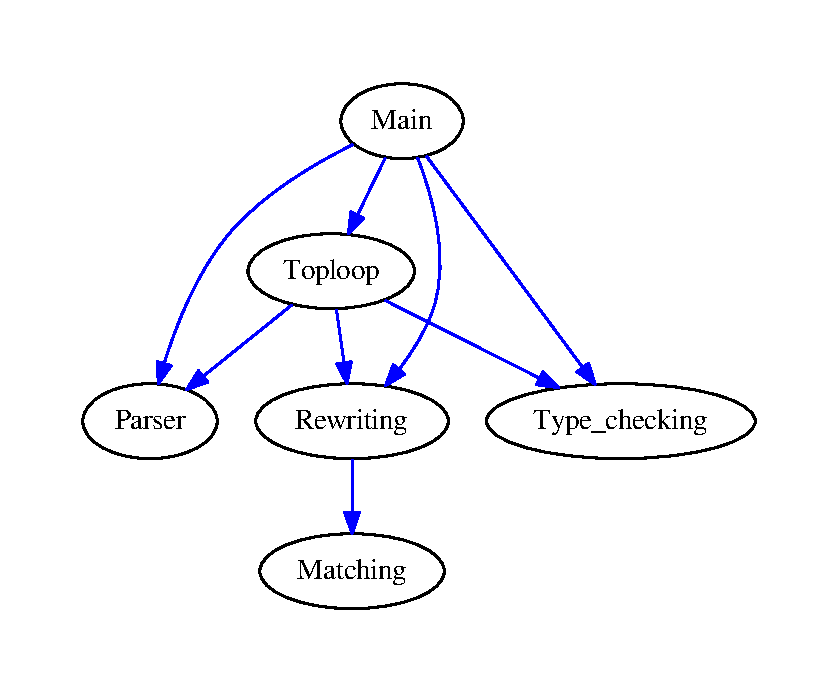
\includegraphics[ height=0.9\textheight]{imports/architecture.pdf}
\end{center}
\end{figure}

\end{frame}


\begin{frame}{Arbres de syntaxe abstraite}

\begin{figure}[h]
\begin{center}
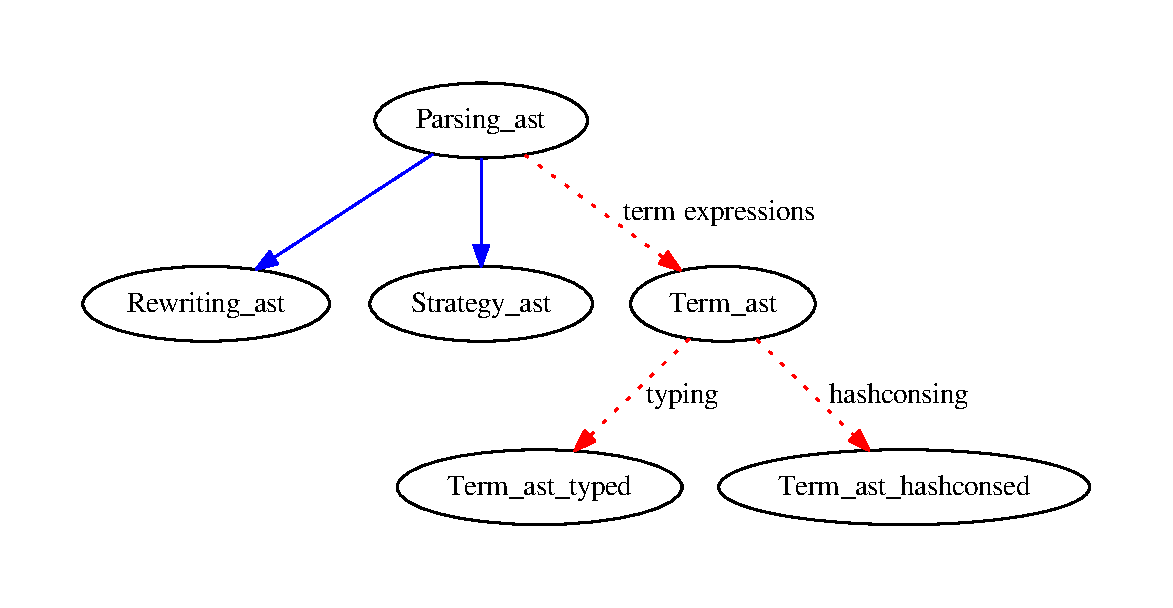
\includegraphics[ height=0.7\textheight]{imports/asts.pdf}
\end{center}
\end{figure}

\end{frame}
